\documentclass[conference]{IEEEtran}
\IEEEoverridecommandlockouts
% The preceding line is only needed to identify funding in the first footnote. If that is unneeded, please comment it out.
\usepackage{cite}
\usepackage{amsmath,amssymb,amsfonts}
\usepackage{algorithmic}
\usepackage{graphicx}
\usepackage{textcomp}
\usepackage{xcolor}
\usepackage[export]{adjustbox}
\usepackage{enumitem}
\usepackage{adjustbox}
\usepackage{subcaption}


\newcommand{\imageitem}[2]{%
  \item
  \begin{adjustbox}{valign=c}
    \includegraphics[width=1cm]{#2} % Adjust the width as needed
  \end{adjustbox}
  \begin{minipage}[t]{\dimexpr\linewidth-1cm\relax}
    #1
  \end{minipage}
}

\def\BibTeX{{\rm B\kern-.05em{\sc i\kern-.025em b}\kern-.08em
    T\kern-.1667em\lower.7ex\hbox{E}\kern-.125emX}}

    \makeatletter
    \newcommand{\linebreakand}{%
      \end{@IEEEauthorhalign}
      \hfill\mbox{}\par
      \mbox{}\hfill\begin{@IEEEauthorhalign}
    }
    \makeatother
\begin{document}


\title{Smart Bus Ticketing and Positioning System\\}


\author{\IEEEauthorblockN{Aditya Singh}
\IEEEauthorblockA{\textit{Dept. of Electronics and Communication} \\
\textit{Dayananda Sagar College of Engineering}\\
Bengaluru, Karnataka, India \\
singhaditya1902@gmail.com} \\
\IEEEauthorblockN{K Vinay Chandra}
\IEEEauthorblockA{\textit{Dept. of Electronics and Communication} \\
\textit{Dayananda Sagar College of Engineering}\\
Bengaluru, Karnataka, India \\
vinaykonda15@gmail.com}
\and
\IEEEauthorblockN{Aman Kumar Jha}
\IEEEauthorblockA{\textit{Dept. of Electronics and Communication} \\
\textit{Dayananda Sagar College of Engineering}\\
Bengaluru, Karnataka, India \\
amank5336@gmail.com} \\
\IEEEauthorblockN{Prof. Shahla Sohail}
\IEEEauthorblockA{\textit{Dept. of Electronics and Communication} \\
\textit{Dayananda Sagar College of Engineering}\\
Bengaluru, Karnataka, India \\
shahla-ece@dayanandasagar.edu}

}

\maketitle

\begin{abstract}
  The Smart Bus System encompasses various functionalities, with its primary feature being the computerized ticket purchasing process [1]. This system comprises two units installed within the bus, positioned at the entry and exit gates. Each unit serves to scan the entry and exit instances of passengers who possess an RFID (Radio Frequency Identification) tag[2], which is read by the RFID reader. Additionally, both units are equipped with GPS modules that continuously update the bus's location at regular intervals, facilitating the tracking of passenger whereabouts during both boarding and disembarking.

  The technology incorporated in this system calculates the fare based on the distance traveled and deducts the corresponding amount from the passenger's E-wallet [3], which can be managed through the S-Bus mobile application. Moreover, the system enables real-time bus tracking, empowering users to plan their trips accordingly. By storing all transactions in a database, the system can analyze the data to determine bus timetables and calculate the required frequency of buses along specific routes. Graphs and live data reception are employed to evaluate daily, weekly, and monthly passenger travel patterns.
  
  In summary, the smart bus system is an efficient, convenient, and highly reliable [3] solution that encompasses automated ticket booking, live bus tracking, and strategic planning and management [1]. By digitizing processes, it promotes a peaceful passenger journey while reducing paper waste and saving time and effort in planning.
  
\end{abstract}

\begin{IEEEkeywords}
    IoT, RFID, Data Analysis, Bus Tracking, Paperless Ticketing
\end{IEEEkeywords}

\section{Introduction}
The Internet of Things (IoT) refers to a network of interconnected devices [2], including cell phones, cars, electrical equipment, and smart sensors [3], which can be monitored and controlled using Big Data technology. This integration of devices brings about improved efficiency, economic benefits, and reduced human involvement. Among various public transportation options, the bus system stands out as a widely used mode of transport.

However, the existing bus system faces challenges in congested metropolitan areas. Lengthy queues and unpredictable waiting times cause significant time wastage for passengers. The lack of accurate tracking systems further complicates matters, as passengers are left unaware of the bus's whereabouts. Additionally, the process of purchasing tickets and dealing with conductors adds frustration for passengers, with issues arising from misunderstandings and the issuance of incorrect tickets.

The extensive use of paper tickets in the bus transit system in India leads to substantial paper waste. These tickets are typically single-use and require daily printing, resulting in a significant amount of paper being discarded each day. Furthermore, the absence of proper analysis systems for bus management leads to inaccuracies in arranging bus timetables. To address these challenges, we propose the implementation of a smart bus system using IoT technology.

By incorporating an RFID reader, the recommended approach enables the automatic scanning of unique tag numbers. The system's processor handles the transaction by deducting the fare from the passenger's RFID tag or card. To provide a digital ticket, an SMS message, referred to as an E-ticket, is sent to the customer/passenger [4], indicating the deducted amount and serving as proof of payment for the specific journey. The timestamp on the message ensures its validity for that particular trip, preventing ticket reuse and mitigating fraudulent activities.
During the coronavirus outbreak, health officials advise individuals to avoid crowded places and limit physical contact with strangers. Public transit users are particularly concerned about this issue. Transport hubs, including stations and airports, are recognized as potential hotspots for infection transmission, with public transport networks being linked to higher virus transmission rates, up to six times greater. Such environments, including airplanes, trains, and buses, create favorable conditions for the spread of droplet-spread viruses like the coronavirus (COVID-19).

To enhance the efficiency of the smart bus system, real-time tracking and monitoring capabilities are integrated [1]. GPS technology is employed to track the exact location of each bus in the fleet. Passengers can access a mobile application or a web portal to view the real-time location of the buses [5], reducing uncertainty and providing accurate estimated arrival times. The smart bus system incorporates data analytics and machine learning algorithms to analyze historical and real-time data. This allows for the optimization of bus routes, scheduling, and resource allocation. By analyzing passenger demand patterns, the system can dynamically adjust bus frequencies and capacities to cater to peak hours and minimize overcrowding.

To encourage passenger engagement and provide a seamless experience, the smart bus system offers various payment options, including contactless payment methods such as mobile wallets or prepaid cards. This eliminates the need for physical cash transactions, reducing the risk of germ transmission and speeding up the boarding process. Integrated passenger information systems are installed on buses, providing real-time updates on routes, schedules, and any service disruptions. This empowers passengers with accurate information, allowing them to plan their journeys more efficiently and make informed decisions.

To address the environmental impact of the transportation sector, the smart bus system promotes sustainability by reducing paper waste [6]. By transitioning to digital tickets and implementing electronic validation systems, the reliance on paper tickets is significantly reduced, contributing to a greener and more eco-friendly public transportation system. The smart bus system also enables seamless integration with other modes of transport, such as metro trains or bike-sharing services. This promotes multimodal transportation and encourages passengers to utilize different modes based on their specific needs, enhancing overall connectivity and reducing congestion on the roads.
\section{Literature Survey}
The work done by Meet J Shah, Rajesh
P Prasad, Aashutosh
S Singh [1] focuses on the system integration of NFC (Near Field Communication) ticketing into an existing public transport infrastructure in Poland. The authors address the need for a more efficient and convenient ticketing system that leverages NFC technology. NFC enables contactless communication between a mobile device and a ticketing terminal, allowing for seamless and convenient ticket validation and payment.

		The authors highlight the benefits of NFC ticketing, such as reduced waiting times, improved passenger flow, and enhanced user experience. They discuss the challenges of integrating NFC technology into an existing infrastructure and propose a solution that takes into account the existing ticketing system in Poland. The findings of the paper emphasize the potential of NFC technology to revolutionize the ticketing process and provide a more efficient and user-friendly experience for public transport users in Poland.

\begin{table}[ht]
\centering
\caption{Summary of Different techniques for Integration of
IoT in Public transport System}
\begin{tabular}{|c|p{2.5cm}|c|p{3cm}|}
\hline
\textbf{S/no} & \textbf{Author} & \textbf{Year} & \textbf{Title/References} \\
\hline
1 & Meet J Shah, Rajesh P Prasad, Aashutosh S Singh & 2020 & System Integration of NFC (Near Field Communication) Ticketing into an Existing Public Transport Infrastructure (existing system in Poland) \\
\hline
2 & Saleem Ulla Shariff, J.C.Narayana Swamy, D Seshachalam & 2016 & Beaglebone black based e-system and advertisement revenue hike scheme for Bangalore city public transportation system \\
\hline
3 & Md. Foisal Mahedi Hasan & 2010 & RFID-based ticketing for public transport system: Perspective megacity Dhaka \\
\hline
\end{tabular}
\end{table}

This research done by [2]	Saleem Ulla Shariff, J.C.Narayana Swamy, Seshachalam [2] presents a Beaglebone Black-based e-system and advertisement revenue hike scheme for the public transportation system in Bangalore city, India. The authors address the need for a technologically advanced system that improves the efficiency and revenue generation of the public transportation system while providing convenience for passengers.

		The paper discusses the implementation of Beaglebone Black, a low-cost, single-board computer, to develop an electronic system for ticketing, passenger information, and advertisement display. The authors propose integrating GPS and GSM modules to track bus locations, provide real-time updates to passengers, and display targeted advertisements on digital signage inside the buses. The findings of the paper suggest that the proposed system can enhance passenger experience, increase revenue through targeted advertisements, and improve operational efficiency in the Bangalore city public transportation system.\\
 In the paper "RFID-based ticketing for public transport system: Perspective megacity Dhaka," Md. Foisal Mahedi Hasan [3] explores the application of RFID technology in the ticketing system of Dhaka, a bustling megacity. The author emphasizes the potential benefits of RFID-based ticketing, such as enhanced efficiency, reduced ticketing fraud, and improved passenger experience. By utilizing RFID tags and readers, the system allows for quick and automated fare deduction, eliminating the need for manual ticket handling. This streamlines the boarding process and reduces queuing times for passengers. The paper discusses the technical aspects of RFID implementation, including tag deployment, reader infrastructure, and system integration. It also addresses the challenges of implementing RFID technology in a complex urban environment like Dhaka, considering factors such as infrastructure requirements, cost-effectiveness, and user acceptance. The findings of the paper shed light on the feasibility and advantages of adopting RFID-based ticketing systems in megacities, providing valuable insights for improving the efficiency of public transport systems.
\section{Methodology}
\begin{figure}[htbp]
    \centering
    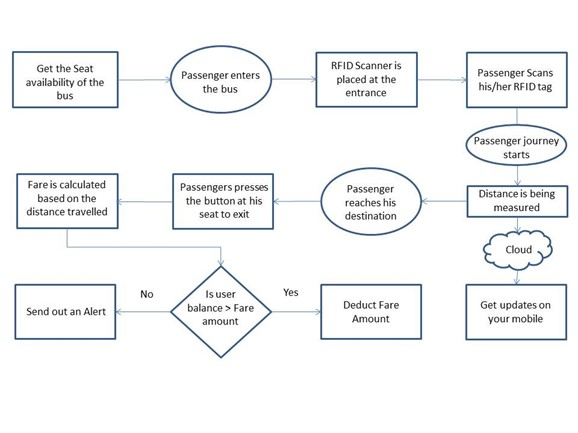
\includegraphics[width=0.8\linewidth]{Picture1.jpg}
    \caption{Flow-chart of the methodology used}
    \label{fig:label_name}
  \end{figure}
  The suggested approach provided here comprises the integration of numerous components to form a full system. The below (Fig. 1) shows the flow chart of the system. The system consists a device that is fitted with RFID, GPS, switches, and a display. Upon activation, the system initializes and awaits a GPS signal to ensure precise location and navigation. Once a GPS signal is captured, the device enters a waiting state for a card to be swiped.
   
  When a genuine card is swiped, the system begins a countdown to mark the start of the voyage. Concurrently, a sensor continually watches for any possible disasters or crises. In the case of such an occurrence, a message is promptly sent to the necessary person responsible for opening the door, guaranteeing timely help and safety precautions.

Continuing under normal conditions, the system continues operating, awaiting a signal from an end switch. When the end switch is triggered, the timer stops, signalling the finish of the adventure or voyage. The distance travelled during the journey is calculated based on the time taken and the speed of the travel. This information is then employed to deduct the necessary amount from the card and send a notification to the individual passenger, presenting them with an updated account balance.

		Additionally, the system integrates infrared sensors to ease seat control. These sensors enable the monitoring of seating capacity and the control of crowds. By leveraging the infrared sensors, the system can efficiently detect the availability of seats and give vital information on seating arrangements.

		Overall, the suggested system demonstrates a smooth integration of numerous technologies to produce a smart and effective trip management system. Through the employment of RFID, GPS, switches, displays, and sensors, the system provides precise location, dependable journey initiation, proactive emergency help, automatic fare deductions, and effective crowd control. This holistic strategy attempts to enhance the whole travel experience by stressing safety, convenience, and operational efficiency.


\section{Proposed System}\label{AA}

In this project, the smart card plays a crucial role in facilitating bus ticket transactions and reservations for each user [7]. The below (Fig. 2) shows us the block diagram of the proposed system. The smart card contains a certain amount of money that can be used exclusively for purchasing bus tickets. As the user boards the bus, they simply slide the card into the smart card reader. Through the utilization of GPS technology, the ticket fare is automatically deducted based on the distance traveled. The GPS receiver provides accurate values that allow the system to calculate the exact distance covered by the user.   
\begin{figure}[htbp]
    \centering
    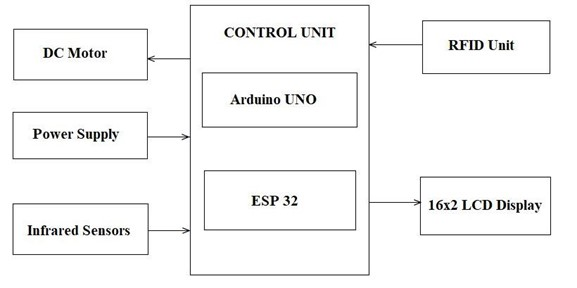
\includegraphics[width=0.8\linewidth]{Picture2.jpg}
    \caption{Block-diagram of the system}
    \label{fig:label_name}
  \end{figure}
  If the balance on the smart card is insufficient to cover the fare, the system denies issuing a ticket. In such cases, the user is required to recharge the same smart card at the bus department to continue using the bus services. When the card balance reaches zero, the system activates a buzzer to alert the user about the lack of funds on the card.

This proposed system can be divided into six key components:

  \begin{enumerate}
    \item \textbf{User Interface: } The user interface serves as the platform for users to interact with the system. It encompasses the smart card reader and other input/output devices that allow users to access various features and functionalities.
    \item \textbf{Smart Card: } Installed on the bus, the smart card reader is responsible for reading the data stored on the smart card. It verifies the balance on the card and enables fare deductions based on the GPS data received from the bus.
    \item \textbf{Smart Card Reader: } Installed on the bus, the smart card reader is responsible for reading the data stored on the smart card. It verifies the balance on the card and enables fare deductions based on the GPS data received from the bus.
    \item \textbf{DC Motor: } Using this we can simulate the movement of the bus. The distance is measured by calculating RPM of the Motor multiplied by Circumference of Tire.
    \item \textbf{Fare Calculation: } Using the distance provided by motor and predefined fare rates, the system calculates the fare based on the distance covered by the user. This ensures that users are charged accurately for their journeys, avoiding any unnecessary costs.
    \item \textbf{Recharge System: } To maintain a seamless user experience, the system provides a recharge mechanism. When the balance on the smart card is insufficient, users can conveniently recharge their cards at the bus department, allowing them to continue using the system without any interruptions or inconveniences.
  \end{enumerate}
  The block diagram of the smart bus ticketing and positioning system incorporates various components to ensure its functionality and efficiency:
  \begin{itemize}
    \item \textbf{ESP32 and Arduino Control Unit: } The ESP32 and Arduino act as the central control unit of the system. They are responsible for receiving inputs from various sensors, processing data, and controlling the overall functionality of the system.
    \begin{figure}[h]
        \centering
        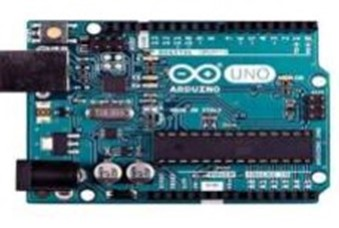
\includegraphics[width=5cm]{uno.jpg} % Replace `image1` with the actual filename of your image
        \caption{Arduino Uno}
      \end{figure}
      \begin{figure}[h]
        \centering
        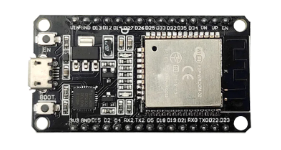
\includegraphics[width=5cm]{esp32.png} % Replace `image1` with the actual filename of your image
        \caption{ESP32}
      \end{figure}
      \item \textbf{IR Sensors: } IR sensors are strategically placed throughout the bus to detect the occupancy status of seats. These sensors can accurately determine whether a seat is occupied or vacant based on the presence or absence of infrared signals. The IR sensor data is sent to the control unit for further processing.
      \begin{figure}[h]
        \centering
        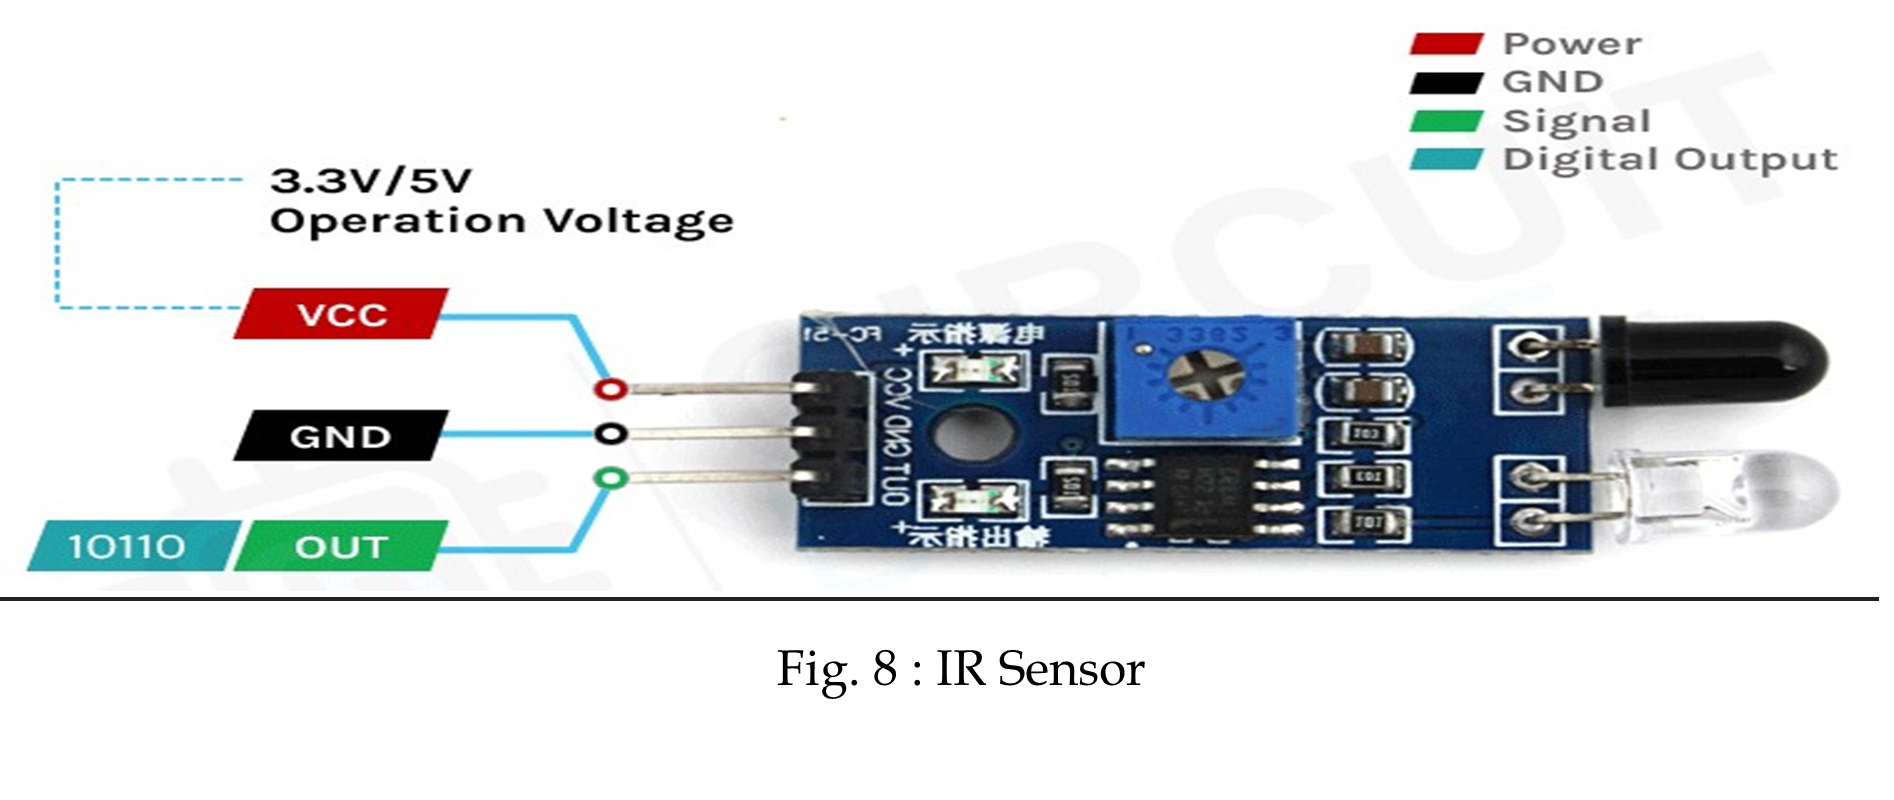
\includegraphics[width=5cm]{ir.png} % Replace `image1` with the actual filename of your image
        \caption{IR Sensor}
      \end{figure}
      \item \textbf{DC Motor: } The DC motor is used to simulate the movement of the bus. By measuring the rotations of the motor, the system can calculate the bus`s speed and distance traveled. The DC motor is connected to the control unit, which receives speed and rotation data from it.
      \begin{figure}[h]
        \centering
        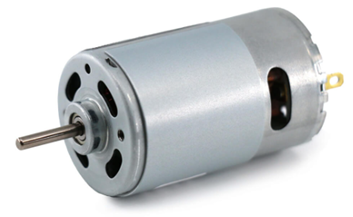
\includegraphics[width=5cm]{motor.png} % Replace `image1` with the actual filename of your image
        \caption{DC Motor}
      \end{figure}
      \item \textbf{16x2 LCD Display: } The LCD display serves as the visual interface for passengers and drivers. It provides essential information such as seat availability status, fare details, and bus location updates. The control unit sends relevant data to the LCD display, which then presents it in a readable format.
      \begin{figure}[h]
        \centering
        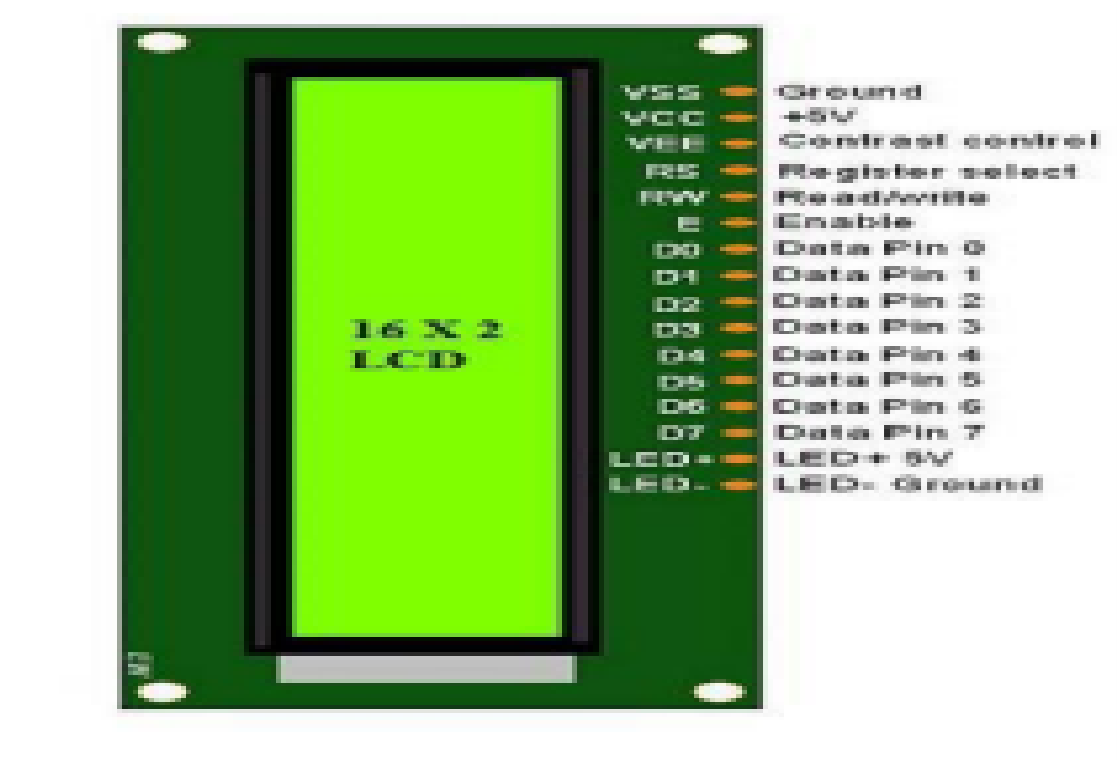
\includegraphics[width=5cm]{lcd.png} % Replace `image1` with the actual filename of your image
        \caption{LCD}
      \end{figure}
      \item \textbf{RFID Cards and RFID Scanner Unit: } Each passenger is provided with an RFID card that contains their payment information and travel history. The RFID scanner unit, located at the entry and exit points of the bus, reads the information stored on the RFID card when it is tapped. The scanner unit communicates with the control unit to update the database with the passenger`s source and destination locations.
      \begin{figure}[h]
        \centering
        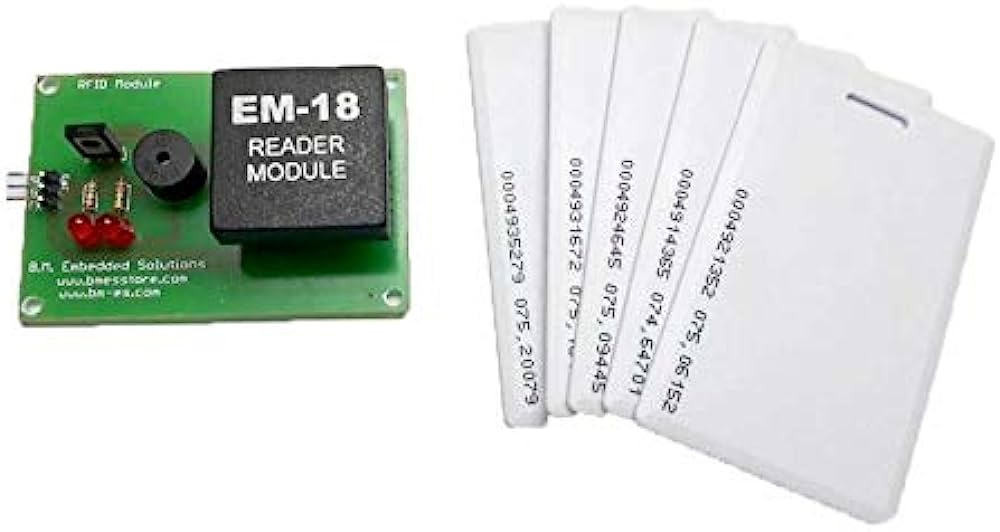
\includegraphics[width=5cm]{rfid.png} % Replace `image1` with the actual filename of your image
        \caption{RFID Scanner and Card}
      \end{figure}
  \end{itemize}

\section{Results}
By implementing RFIDs, our system enables convenient cashless transactions and eliminates the need for physical tickets when traveling on a bus. Using the distance obtained by DC Motor and IR Sensor, we can charge a fair amount by using a base amount for each km of distance. The User can see if there are any seats available or not and fare details on a Telegram Bot.
Incorporating a distance calculation program, we accurately determine the distance traveled by users and calculate fares accordingly. This ensures that passengers are charged fairly, eliminating any unnecessary expenses.
\begin{figure}[!htb]
    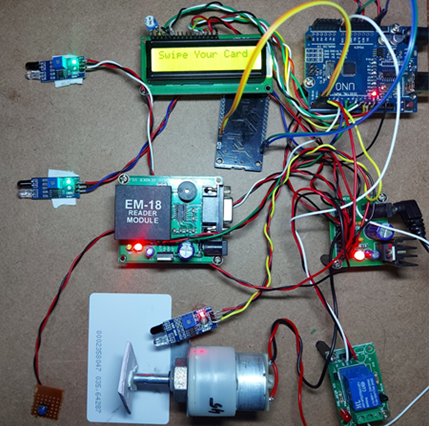
\includegraphics[width=.4\linewidth]{r1.png}\hfill
    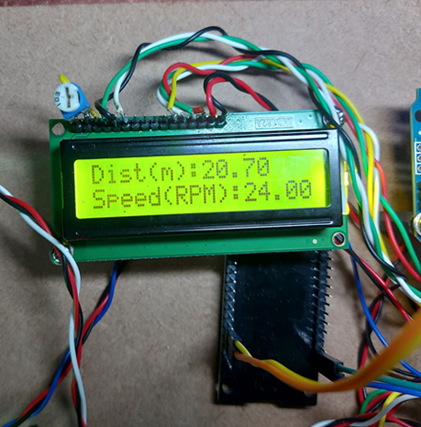
\includegraphics[width=.4\linewidth]{r2.png}
    \caption{Prototype Results}\label{fig:foobar}
\end{figure}

\section{conclusion and future work}
The proposed system aims to achieve full automation, reliability, transparency, convenience, and effectiveness in transportation facilities. This model has been successfully implemented in numerous developed countries, showcasing its potential for improving transport systems. As an emerging country, we have the opportunity to adopt and implement an efficient transport system.

The integration of automatic ticket systems brings significant benefits to operators, such as transportation authorities. It allows them to save time and reduce personal costs, as fare collection can be streamlined and managed more efficiently. Moreover, these systems offer advantages of low maintenance costs and minimize losses resulting from fraudulent activities.

Furthermore, the proposed system can be extended to include the railway ticketing system. By utilizing reusable cards, it offers enhanced convenience compared to traditional paper-based ticketing methods. This not only simplifies the ticketing process for passengers but also reduces paper waste and contributes to environmental sustainability. By embracing such advanced ticketing systems, we can optimize our transport infrastructure and enhance the overall passenger experience, aligning with global standards and best practices.

The smart bus ticketing system project has a promising scope for future work. One area of focus is the integration of a mobile application that connects to the ESP32 via its inbuilt WiFi module. This mobile app will enable users to access real-time bus location, track their journey, view fare details, and make cashless payments, providing a convenient and user-friendly experience.
Collaboration with local transit authorities, obtaining their support, and ensuring compliance with existing transportation systems will be crucial in expanding the project`s reach and impact. Lastly, gathering user feedback and continuously improving the system based on user suggestions and concerns will contribute to higher user satisfaction and a better overall experience.
Overall, by pursuing these future developments, the smart bus ticketing system can evolve into a comprehensive solution, offering enhanced convenience, efficiency, and security to both passengers and transportation authorities.




\begin{thebibliography}{99}
  
\bibitem{ref1} J. Shah, R. P. Prasad, A. S. Singh. "IOT Based Smart Bus System", 2020 3rd International Conference on Communication System, Computing and IT Applications (CSCITA), 2020.

\bibitem{ref2} M. G. Gnoni, A. Rollo, P. Tundo. "A smart model for urban ticketing based on RFID applications," P-0572, 2009 IEEE International.

\bibitem{ref3} S. U. Shariff, J. C. Narayana Swamy, Seshachalam. "Beaglebone black based e-system and advertisement revenue hike scheme for Bangalore city public transportation system", 2016 2nd International Conference on Applied and Theoretical Computing and Communication Technology (iCATccT), 2016.

\bibitem{ref4} Md. F. M. Hasan. "RFID-based ticketing for public transport system: Perspective megacity Dhaka", 2010 3rd International Conference on Computer Science and Information Technology, 07/2010.

\bibitem{ref5} R. Widmann. "System Integration of NFC Ticketing into an Existing Public Transport Infrastructure", 2012 4th International.

\bibitem{ref6} S. B. Arniker, K. S. Rama Rao, G. Kalyani, D. Meena, M. Lalitha, K. Shirisha, S. Seetasaikiran. "RFID based missing person identification system", 2014 International Conference on Informatics, Electronics \& Vision (ICIEV), 2014.

\bibitem{ref7} D. Iwanowicz, T. Szczuraszek. "Concept of A System for Integrated Ticketing and Tariffs for A Given Area in Poland", IOP Conference Series: Materials Science and Engineering, 2019.

\bibitem{ref8} Y. F. Yan, S. F. Zhang, Y. H. Zhang, F. G. Zuo, F. D. Li. "Design of Network Power Meter Based on Modbus TCP", Applied Mechanics and Materials, 2013.

\bibitem{ref9} A. Datta, K. Raj, R. Sarker. "Implementation of a high accuracy ac current sensing scheme using hall-sensor", 2019 International Conference on Energy Management for Green Environment (UEMGREEN), 2019.

\bibitem{ref10} B. Malakar, B. K. Roy. "Survey of RFID applications in railway industry", 2014 First International Conference on Automation Control Energy and Systems (ACES), 2014.

\bibitem{ref11} W. Maslak, B. S. Butkiewicz. "Autonomous vehicle with fuzzy control", 2013 Signal Processing Symposium (SPS), 2013.

\bibitem{ref12} P. Daly. "Navstar GPS and GLONASS: global satellite navigation systems", Electronics and Communication Engg., July 2005.

\bibitem{ref13} S. Garfinkal, B. Rosenberg. "RFID: Application, Security \& Privacy", Addison Wesley Professional, Upper Saddle Rider, Edition 2005.

\bibitem{ref14} S. Hodges, D. McFarlance. "RFID: Technology, Application \& Impact", 2005.

\bibitem{ref15} S. Gopi. "Global Positioning System: Principles and Application", Tata McGraw-Hill Education, 2005.

\bibitem{ref16} V. K. Garg. "Principles and Applications of GSM", 1998, Mc Graw Hills Publication.

\bibitem{ref17} M. A. Mazidi, R. D. McKinlay, D. Causey. "P89V51 Microcontroller and Embedded Systems Using Assembly and C for P89V51", Pearson Education, 2008.

\bibitem{ref18} B. Yan, D. Lee. "Ticketing System Based on RFID", 2009 International Conference on Networks Security, Wireless Communications and Trusted Computing.

\end{thebibliography}




\end{document}
